\documentclass[twoside]{article}

% Packages required by doxygen
\usepackage{fixltx2e}
\usepackage{calc}
\usepackage{doxygen}
\usepackage[export]{adjustbox} % also loads graphicx
\usepackage{graphicx}
\usepackage[utf8]{inputenc}
\usepackage{makeidx}
\usepackage{multicol}
\usepackage{multirow}
\PassOptionsToPackage{warn}{textcomp}
\usepackage{textcomp}
\usepackage[nointegrals]{wasysym}
\usepackage[table]{xcolor}

% Font selection
\usepackage[T1]{fontenc}
\usepackage[scaled=.90]{helvet}
\usepackage{courier}
\usepackage{amssymb}
\usepackage{sectsty}
\renewcommand{\familydefault}{\sfdefault}
\allsectionsfont{%
  \fontseries{bc}\selectfont%
  \color{darkgray}%
}
\renewcommand{\DoxyLabelFont}{%
  \fontseries{bc}\selectfont%
  \color{darkgray}%
}
\newcommand{\+}{\discretionary{\mbox{\scriptsize$\hookleftarrow$}}{}{}}

% Page & text layout
\usepackage{geometry}
\geometry{%
  a4paper,%
  top=2.5cm,%
  bottom=2.5cm,%
  left=2.5cm,%
  right=2.5cm%
}
\tolerance=750
\hfuzz=15pt
\hbadness=750
\setlength{\emergencystretch}{15pt}
\setlength{\parindent}{0cm}
\setlength{\parskip}{3ex plus 2ex minus 2ex}
\makeatletter
\renewcommand{\paragraph}{%
  \@startsection{paragraph}{4}{0ex}{-1.0ex}{1.0ex}{%
    \normalfont\normalsize\bfseries\SS@parafont%
  }%
}
\renewcommand{\subparagraph}{%
  \@startsection{subparagraph}{5}{0ex}{-1.0ex}{1.0ex}{%
    \normalfont\normalsize\bfseries\SS@subparafont%
  }%
}
\makeatother

% Headers & footers
\usepackage{fancyhdr}
\pagestyle{fancyplain}
\fancyhead[LE]{\fancyplain{}{\bfseries\thepage}}
\fancyhead[CE]{\fancyplain{}{}}
\fancyhead[RE]{\fancyplain{}{\bfseries\leftmark}}
\fancyhead[LO]{\fancyplain{}{\bfseries\rightmark}}
\fancyhead[CO]{\fancyplain{}{}}
\fancyhead[RO]{\fancyplain{}{\bfseries\thepage}}
\fancyfoot[LE]{\fancyplain{}{}}
\fancyfoot[CE]{\fancyplain{}{}}
\fancyfoot[RE]{\fancyplain{}{\bfseries\scriptsize Generated by Doxygen }}
\fancyfoot[LO]{\fancyplain{}{\bfseries\scriptsize Generated by Doxygen }}
\fancyfoot[CO]{\fancyplain{}{}}
\fancyfoot[RO]{\fancyplain{}{}}
\renewcommand{\footrulewidth}{0.4pt}
\renewcommand{\sectionmark}[1]{%
  \markright{\thesection\ #1}%
}

% Indices & bibliography
\usepackage{natbib}
\usepackage[titles]{tocloft}
\setcounter{tocdepth}{3}
\setcounter{secnumdepth}{5}
\makeindex

% Hyperlinks (required, but should be loaded last)
\usepackage{ifpdf}
\ifpdf
  \usepackage[pdftex,pagebackref=true]{hyperref}
\else
  \usepackage[ps2pdf,pagebackref=true]{hyperref}
\fi
\hypersetup{%
  colorlinks=true,%
  linkcolor=blue,%
  citecolor=blue,%
  unicode%
}

% Custom commands
\newcommand{\clearemptydoublepage}{%
  \newpage{\pagestyle{empty}\cleardoublepage}%
}

\usepackage{caption}
\captionsetup{labelsep=space,justification=centering,font={bf},singlelinecheck=off,skip=4pt,position=top}

%===== C O N T E N T S =====

\begin{document}

% Titlepage & ToC
\hypersetup{pageanchor=false,
             bookmarksnumbered=true,
             pdfencoding=unicode
            }
\pagenumbering{alph}
\begin{titlepage}
\vspace*{7cm}
\begin{center}%
{\Large Diagrams }\\
\vspace*{1cm}
{\large Generated by Doxygen 1.8.12}\\
\end{center}
\end{titlepage}
\pagenumbering{roman}
\tableofcontents
\pagenumbering{arabic}
\hypersetup{pageanchor=true}

%--- Begin generated contents ---
\section{Class Documentation}
\hypertarget{class_a}{}\subsection{A Class Reference}
\label{class_a}\index{A@{A}}


{\ttfamily \#include $<$diagrams\+\_\+a.\+h$>$}



Inheritance diagram for A\+:
\nopagebreak
\begin{figure}[H]
\begin{center}
\leavevmode
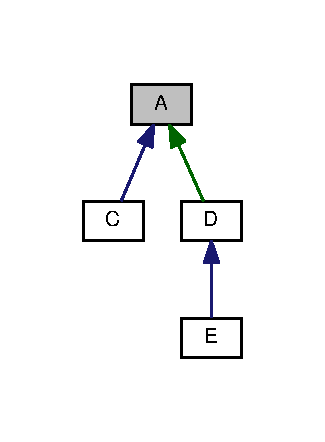
\includegraphics[width=156pt]{class_a__inherit__graph}
\end{center}
\end{figure}


Collaboration diagram for A\+:
\nopagebreak
\begin{figure}[H]
\begin{center}
\leavevmode
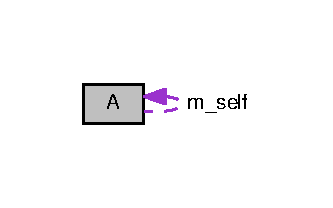
\includegraphics[width=160pt]{class_a__coll__graph}
\end{center}
\end{figure}
\subsubsection*{Public Attributes}
\begin{DoxyCompactItemize}
\item 
\hyperlink{class_a}{A} $\ast$ \hyperlink{class_a_a086d3a4efc697dba0601b9fef3d082ad}{m\+\_\+self}
\end{DoxyCompactItemize}


\subsubsection{Member Data Documentation}
\hypertarget{class_a_a086d3a4efc697dba0601b9fef3d082ad}{}\label{class_a_a086d3a4efc697dba0601b9fef3d082ad} 
\index{A@{A}!m\+\_\+self@{m\+\_\+self}}
\index{m\+\_\+self@{m\+\_\+self}!A@{A}}
\paragraph{\texorpdfstring{m\+\_\+self}{m\_self}}
{\footnotesize\ttfamily \hyperlink{class_a}{A}$\ast$ A\+::m\+\_\+self}



The documentation for this class was generated from the following file\+:\begin{DoxyCompactItemize}
\item 
\hyperlink{diagrams__a_8h}{diagrams\+\_\+a.\+h}\end{DoxyCompactItemize}

\hypertarget{class_b}{}\subsection{B Class Reference}
\label{class_b}\index{B@{B}}


{\ttfamily \#include $<$diagrams\+\_\+b.\+h$>$}



Inheritance diagram for B\+:
\nopagebreak
\begin{figure}[H]
\begin{center}
\leavevmode
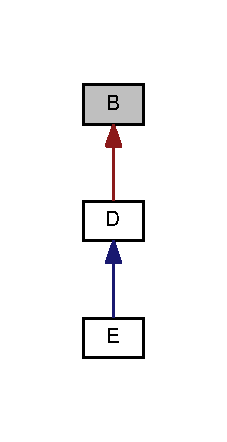
\includegraphics[width=109pt]{class_b__inherit__graph}
\end{center}
\end{figure}


Collaboration diagram for B\+:
\nopagebreak
\begin{figure}[H]
\begin{center}
\leavevmode
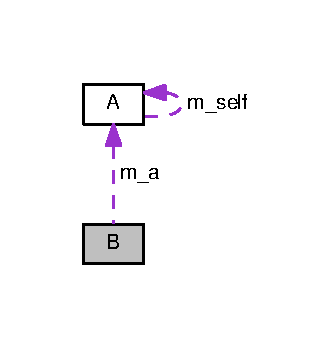
\includegraphics[width=160pt]{class_b__coll__graph}
\end{center}
\end{figure}
\subsubsection*{Public Attributes}
\begin{DoxyCompactItemize}
\item 
\hyperlink{class_a}{A} $\ast$ \hyperlink{class_b_a26c70b64fe7cf17fcced7755ecff7537}{m\+\_\+a}
\end{DoxyCompactItemize}


\subsubsection{Member Data Documentation}
\hypertarget{class_b_a26c70b64fe7cf17fcced7755ecff7537}{}\label{class_b_a26c70b64fe7cf17fcced7755ecff7537} 
\index{B@{B}!m\+\_\+a@{m\+\_\+a}}
\index{m\+\_\+a@{m\+\_\+a}!B@{B}}
\paragraph{\texorpdfstring{m\+\_\+a}{m\_a}}
{\footnotesize\ttfamily \hyperlink{class_a}{A}$\ast$ B\+::m\+\_\+a}



The documentation for this class was generated from the following file\+:\begin{DoxyCompactItemize}
\item 
\hyperlink{diagrams__b_8h}{diagrams\+\_\+b.\+h}\end{DoxyCompactItemize}

\hypertarget{class_c}{}\subsection{C Class Reference}
\label{class_c}\index{C@{C}}


{\ttfamily \#include $<$diagrams\+\_\+c.\+h$>$}



Inheritance diagram for C\+:
\nopagebreak
\begin{figure}[H]
\begin{center}
\leavevmode
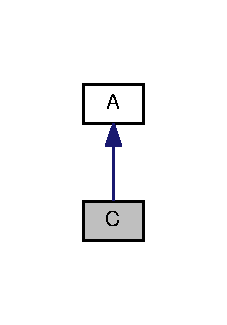
\includegraphics[width=109pt]{class_c__inherit__graph}
\end{center}
\end{figure}


Collaboration diagram for C\+:
\nopagebreak
\begin{figure}[H]
\begin{center}
\leavevmode
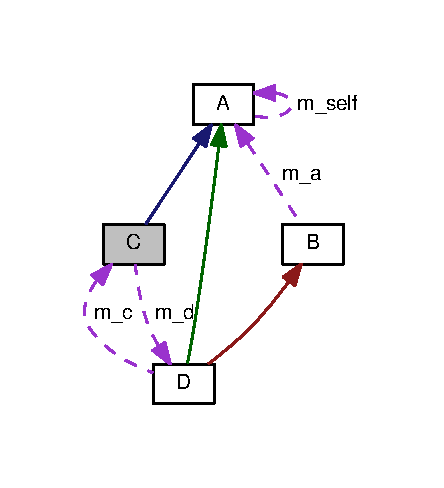
\includegraphics[width=213pt]{class_c__coll__graph}
\end{center}
\end{figure}
\subsubsection*{Public Attributes}
\begin{DoxyCompactItemize}
\item 
\hyperlink{class_d}{D} $\ast$ \hyperlink{class_c_a4ef972d28b73ff78eba3ab4f54c3b449}{m\+\_\+d}
\end{DoxyCompactItemize}


\subsubsection{Member Data Documentation}
\hypertarget{class_c_a4ef972d28b73ff78eba3ab4f54c3b449}{}\label{class_c_a4ef972d28b73ff78eba3ab4f54c3b449} 
\index{C@{C}!m\+\_\+d@{m\+\_\+d}}
\index{m\+\_\+d@{m\+\_\+d}!C@{C}}
\paragraph{\texorpdfstring{m\+\_\+d}{m\_d}}
{\footnotesize\ttfamily \hyperlink{class_d}{D}$\ast$ C\+::m\+\_\+d}



The documentation for this class was generated from the following file\+:\begin{DoxyCompactItemize}
\item 
\hyperlink{diagrams__c_8h}{diagrams\+\_\+c.\+h}\end{DoxyCompactItemize}

\hypertarget{class_d}{}\subsection{D Class Reference}
\label{class_d}\index{D@{D}}


{\ttfamily \#include $<$diagrams\+\_\+d.\+h$>$}



Inheritance diagram for D\+:
\nopagebreak
\begin{figure}[H]
\begin{center}
\leavevmode
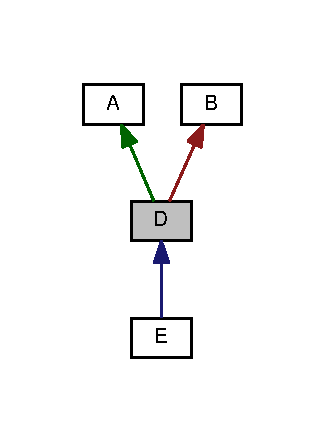
\includegraphics[width=156pt]{class_d__inherit__graph}
\end{center}
\end{figure}


Collaboration diagram for D\+:
\nopagebreak
\begin{figure}[H]
\begin{center}
\leavevmode
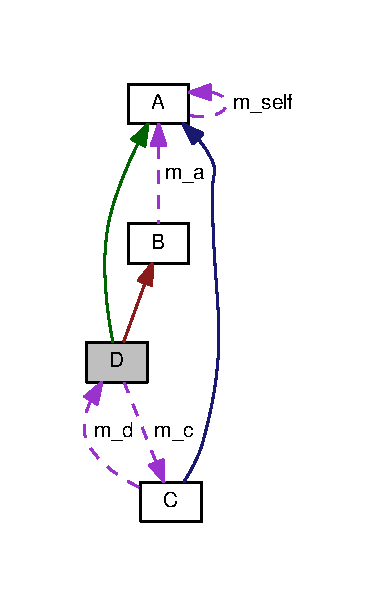
\includegraphics[width=182pt]{class_d__coll__graph}
\end{center}
\end{figure}
\subsubsection*{Public Attributes}
\begin{DoxyCompactItemize}
\item 
\hyperlink{class_c}{C} \hyperlink{class_d_a9d877c7aa092f423f2a073f3c62fef9c}{m\+\_\+c}
\end{DoxyCompactItemize}
\subsubsection*{Additional Inherited Members}


\subsubsection{Member Data Documentation}
\hypertarget{class_d_a9d877c7aa092f423f2a073f3c62fef9c}{}\label{class_d_a9d877c7aa092f423f2a073f3c62fef9c} 
\index{D@{D}!m\+\_\+c@{m\+\_\+c}}
\index{m\+\_\+c@{m\+\_\+c}!D@{D}}
\paragraph{\texorpdfstring{m\+\_\+c}{m\_c}}
{\footnotesize\ttfamily \hyperlink{class_c}{C} D\+::m\+\_\+c}



The documentation for this class was generated from the following file\+:\begin{DoxyCompactItemize}
\item 
\hyperlink{diagrams__d_8h}{diagrams\+\_\+d.\+h}\end{DoxyCompactItemize}

\hypertarget{class_e}{}\subsection{E Class Reference}
\label{class_e}\index{E@{E}}


{\ttfamily \#include $<$diagrams\+\_\+e.\+h$>$}



Inheritance diagram for E\+:
\nopagebreak
\begin{figure}[H]
\begin{center}
\leavevmode
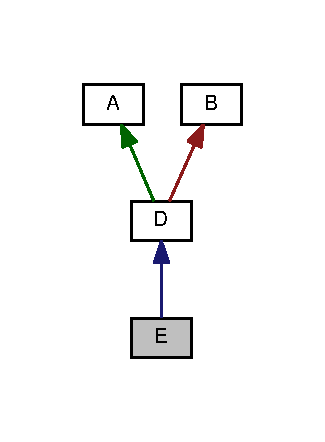
\includegraphics[width=156pt]{class_e__inherit__graph}
\end{center}
\end{figure}


Collaboration diagram for E\+:
\nopagebreak
\begin{figure}[H]
\begin{center}
\leavevmode
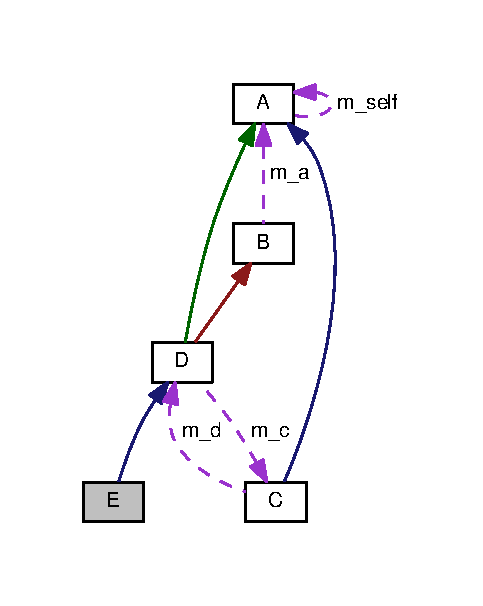
\includegraphics[width=232pt]{class_e__coll__graph}
\end{center}
\end{figure}
\subsubsection*{Additional Inherited Members}


The documentation for this class was generated from the following file\+:\begin{DoxyCompactItemize}
\item 
\hyperlink{diagrams__e_8h}{diagrams\+\_\+e.\+h}\end{DoxyCompactItemize}

\section{File Documentation}
\hypertarget{diagrams__a_8h}{}\subsection{diagrams\+\_\+a.\+h File Reference}
\label{diagrams__a_8h}\index{diagrams\+\_\+a.\+h@{diagrams\+\_\+a.\+h}}
This graph shows which files directly or indirectly include this file\+:
\nopagebreak
\begin{figure}[H]
\begin{center}
\leavevmode
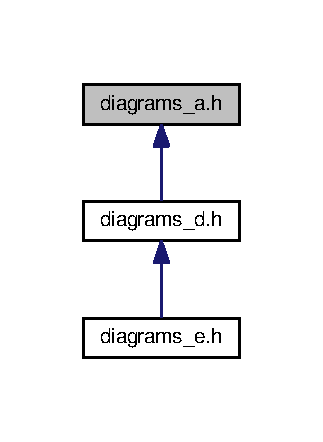
\includegraphics[width=155pt]{diagrams__a_8h__dep__incl}
\end{center}
\end{figure}
\subsubsection*{Classes}
\begin{DoxyCompactItemize}
\item 
class \hyperlink{class_a}{A}
\end{DoxyCompactItemize}

\hypertarget{diagrams__b_8h}{}\subsection{diagrams\+\_\+b.\+h File Reference}
\label{diagrams__b_8h}\index{diagrams\+\_\+b.\+h@{diagrams\+\_\+b.\+h}}
This graph shows which files directly or indirectly include this file\+:
\nopagebreak
\begin{figure}[H]
\begin{center}
\leavevmode
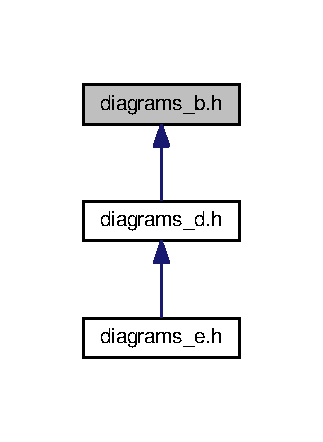
\includegraphics[width=155pt]{diagrams__b_8h__dep__incl}
\end{center}
\end{figure}
\subsubsection*{Classes}
\begin{DoxyCompactItemize}
\item 
class \hyperlink{class_b}{B}
\end{DoxyCompactItemize}

\hypertarget{diagrams__c_8h}{}\subsection{diagrams\+\_\+c.\+h File Reference}
\label{diagrams__c_8h}\index{diagrams\+\_\+c.\+h@{diagrams\+\_\+c.\+h}}
{\ttfamily \#include \char`\"{}diagrams\+\_\+c.\+h\char`\"{}}\newline
Include dependency graph for diagrams\+\_\+c.\+h\+:
\nopagebreak
\begin{figure}[H]
\begin{center}
\leavevmode
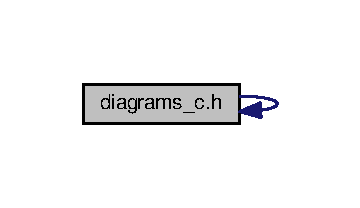
\includegraphics[width=173pt]{diagrams__c_8h__incl}
\end{center}
\end{figure}
This graph shows which files directly or indirectly include this file\+:
\nopagebreak
\begin{figure}[H]
\begin{center}
\leavevmode
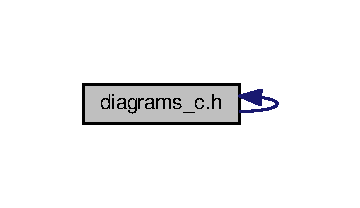
\includegraphics[width=173pt]{diagrams__c_8h__dep__incl}
\end{center}
\end{figure}
\subsubsection*{Classes}
\begin{DoxyCompactItemize}
\item 
class \hyperlink{class_c}{C}
\end{DoxyCompactItemize}

\hypertarget{diagrams__d_8h}{}\subsection{diagrams\+\_\+d.\+h File Reference}
\label{diagrams__d_8h}\index{diagrams\+\_\+d.\+h@{diagrams\+\_\+d.\+h}}
{\ttfamily \#include \char`\"{}diagrams\+\_\+a.\+h\char`\"{}}\newline
{\ttfamily \#include \char`\"{}diagrams\+\_\+b.\+h\char`\"{}}\newline
Include dependency graph for diagrams\+\_\+d.\+h\+:
\nopagebreak
\begin{figure}[H]
\begin{center}
\leavevmode
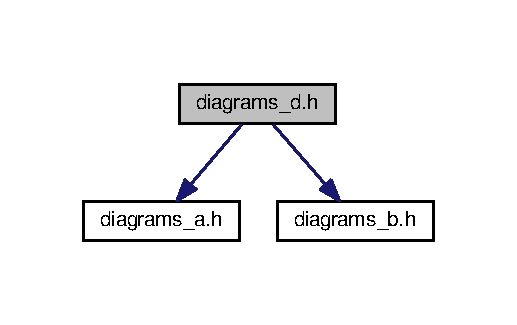
\includegraphics[width=248pt]{diagrams__d_8h__incl}
\end{center}
\end{figure}
This graph shows which files directly or indirectly include this file\+:
\nopagebreak
\begin{figure}[H]
\begin{center}
\leavevmode
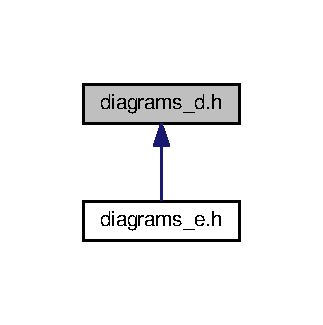
\includegraphics[width=155pt]{diagrams__d_8h__dep__incl}
\end{center}
\end{figure}
\subsubsection*{Classes}
\begin{DoxyCompactItemize}
\item 
class \hyperlink{class_d}{D}
\end{DoxyCompactItemize}

\hypertarget{diagrams__e_8h}{}\subsection{diagrams\+\_\+e.\+h File Reference}
\label{diagrams__e_8h}\index{diagrams\+\_\+e.\+h@{diagrams\+\_\+e.\+h}}
{\ttfamily \#include \char`\"{}diagrams\+\_\+d.\+h\char`\"{}}\newline
Include dependency graph for diagrams\+\_\+e.\+h\+:
\nopagebreak
\begin{figure}[H]
\begin{center}
\leavevmode
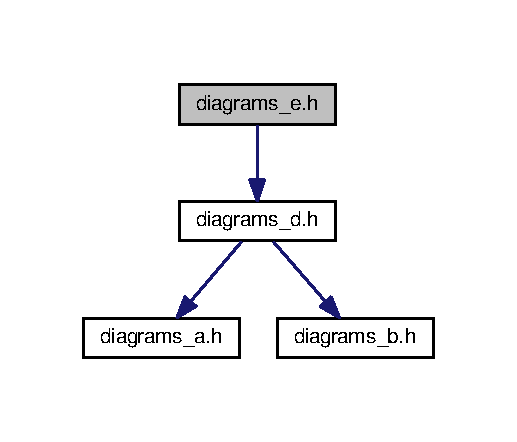
\includegraphics[width=248pt]{diagrams__e_8h__incl}
\end{center}
\end{figure}
\subsubsection*{Classes}
\begin{DoxyCompactItemize}
\item 
class \hyperlink{class_e}{E}
\end{DoxyCompactItemize}

%--- End generated contents ---

% Index
\newpage
\phantomsection
\clearemptydoublepage
\addcontentsline{toc}{section}{Index}
\printindex

\end{document}
